\section{Integration Strategy} \label{sec:intstra}

\subsection{Entry Criteria}
%Specify the criteria that must be met before integration testing of specific elements may begin (e.g., functions must have been unit tested).

In this part of the document, we are going to specify the criteria that must be met before integration testing of specific elements may begin:

\begin{itemize}

\item[\textbf{--}] The \acl{rasd} and the \acl{dd} must be already completed, in order to know the interaction of the various components and their expected behaviour;

\item[\textbf{--}] Each component of our software must have successfully passed the Unit Testing;

\item[\textbf{--}] So, the correct version of our application is moved into the integration testing environment;

\item[\textbf{--}] All the code of our project must be already written and so the major functionality must be present;

\item[\textbf{--}] Our project should satisfy the memory requirements specified in the \acs{rasd};

\item[\textbf{--}] The database should be ready and its tables should already be populated with the initial data.

\end{itemize}

\subsection{Elements to be Integrated}
%Identify the components to be integrated,refer to your design document to identify such components in a way that is consistent with your design.

As we have shown in the \acl{dd} related to our project PowerEnJoy, the system relies on many high-level components, each one implementing a specific set of functionalities, that interacts between them.
Since we have decide to follow a modular approach, each components is the result of the combination of various subcomponents.
However, since we haven't fully defined all low level component needed for our system, we think it is better to focus our integration testing only on the Business Logic and its components (for further information, see \textit{Section 2} of the \acl{dd}). By doing this choice, we have to consider that, in the following evolution of our project, the needed subcomponents will be created and further \acl{it} must be carried out.
 
So, for what we said above, the elements to be integrated are the following:

\begin{itemize}

\item[\textbf{--}] Web Component and Business Logic Component, testing the  direct connections between Managed Beans and their corresponding Managers;

\item[\textbf{--}] the subcomponents of the Business Logic Component, integrating them, each one with the needed others.

\end{itemize}

\subsection{Integration Testing Strategy}
%Describe the integration testing approach(top-­‐down, bottom-­‐up, functional groupings,etc.) and the rationale for the choosing that approach.
As we explained above, in this stage of the development we haven't fully defined the hierarchy of all subcomponents and subsystem.
For this reason, we will have an \acl{it} strategy for a single abstract layer and we have to keep in mind that other lower level subcomponents will be implemented.
Although it is not possible to define the final integration test strategy, we think that, as far as we know at this stage, the better strategy we can apply is the top-down approach.
Moreover, the chose of this strategy allow us to test the new subcomponent folowing the downward development.

\subsection{Sequence of Component/Function Integration}
%NOTE: The structure of this section may vary depending on the integration strategy you select in Section 2.3; use the structure proposed below as a non mandatory guide

\vspace{40pt}

\begin{figure}[htbp]
\centering
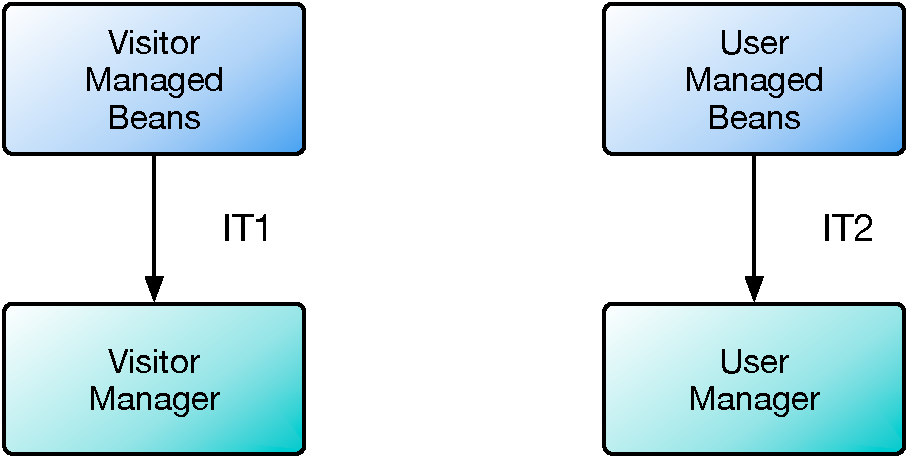
\includegraphics[width=0.6\textwidth]{Images/IT1-2.pdf}
\vspace{16pt}
\caption{Managed Beans and corresponding Managers connections}
\label{fig:it1-2}
\end{figure}

\vspace{16pt}

\begin{table}[htbp]
\begin{center}
\begin{tabular}[t]{cccc}

\hline
\textbf{ID} & \textbf{Components} & \textbf{\acs{it}} & \textbf{\acs{tp}}\\
\hline
IT1 & \enspace Visitor Managed Beans $\rightarrow$ Visitor Manager \enspace & \ref{sssec:IT1} & \ref{sssec:TP1}\\
\hline
IT2 & \enspace User Managed Beans $\rightarrow$ User Manager \enspace & \ref{sssec:IT2} & 
\ref{sssec:TP1}\\
\hline

\end{tabular}
\caption{Managed Beans and corresponding Managers connections}
\end{center}
\end{table}

\clearpage

\vspace{120pt}
\begin{figure}[htbp]
\centering
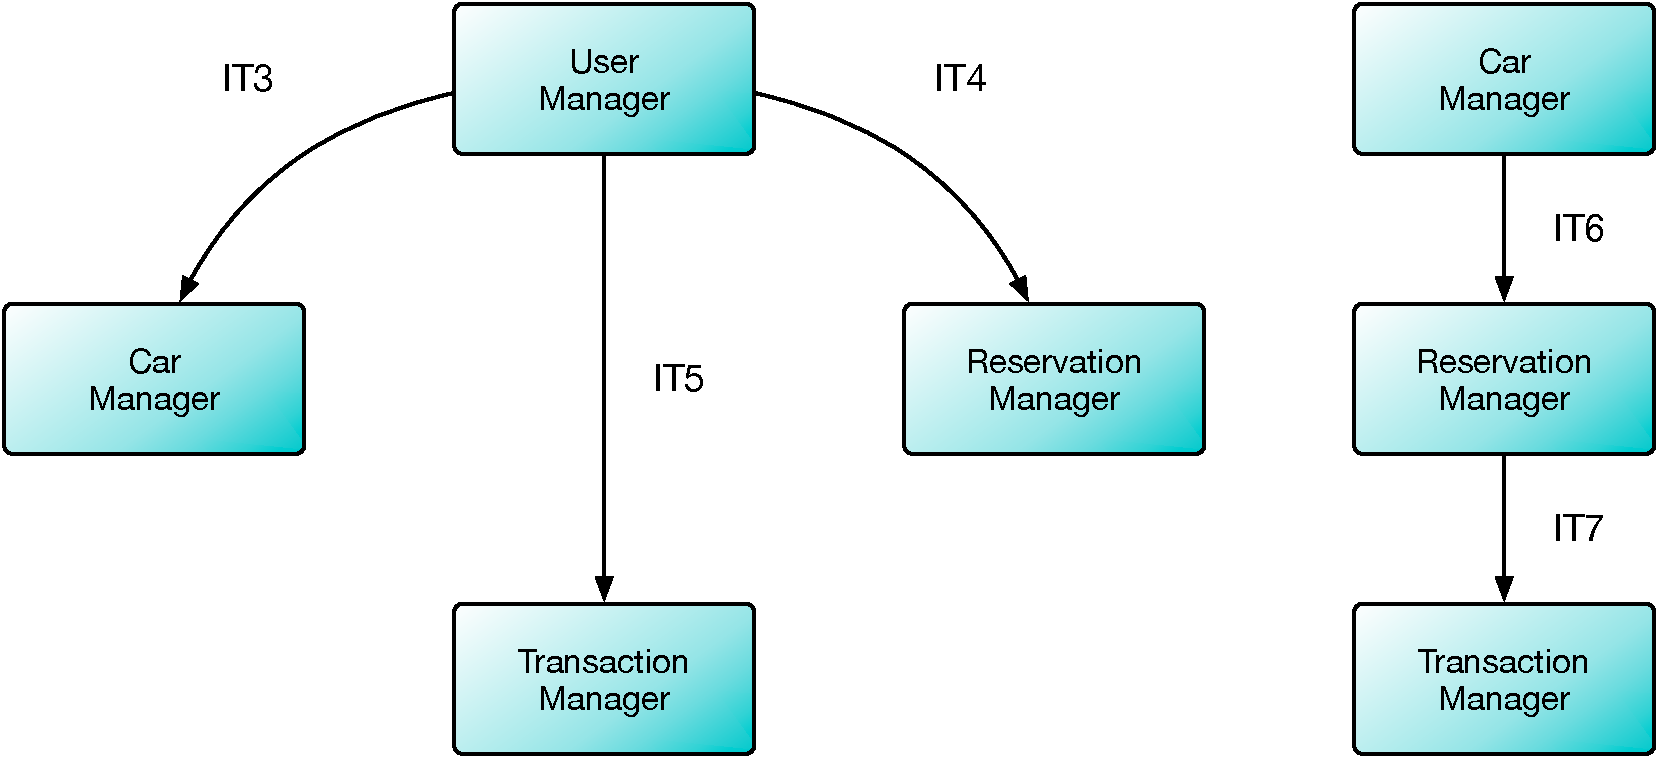
\includegraphics[width=\textwidth]{Images/IT3-7.pdf}
\vspace{16pt}
\caption{Business-tier subcomponents connections}
\label{fig:it3-7}
\end{figure}

\vspace{16pt}

\begin{table}[htbp]
\begin{center}
\begin{tabular}[t]{cccc}

\hline
\textbf{ID} & \textbf{Components} & \textbf{\acs{it}} & \textbf{\acs{tp}}\\
\hline
IT3 & \enspace User Manager $\rightarrow$ Car Manager \enspace & \ref{sssec:IT3} & \ref{sssec:TP2}\\
\hline
IT4 & \enspace User Manager $\rightarrow$ Reservation Manager \enspace & \ref{sssec:IT4} & \ref{sssec:TP2}\\
\hline
IT5 & \enspace User Manager $\rightarrow$ Transaction Manager \enspace & \ref{sssec:IT5} & \ref{sssec:TP2}\\
\hline
IT6 & \enspace Car Manager $\rightarrow$ Reservation Manager \enspace & \ref{sssec:IT6} & \ref{sssec:TP2}\\
\hline
IT7 & \enspace Reservation Manager $\rightarrow$ Transaction Manager \enspace & \ref{sssec:IT7} & \ref{sssec:TP2}\\
\hline


\end{tabular}
\caption{Business-tier subcomponents connections}
\end{center}
\end{table}

\clearpage

\begin{figure}[htbp]
\centering
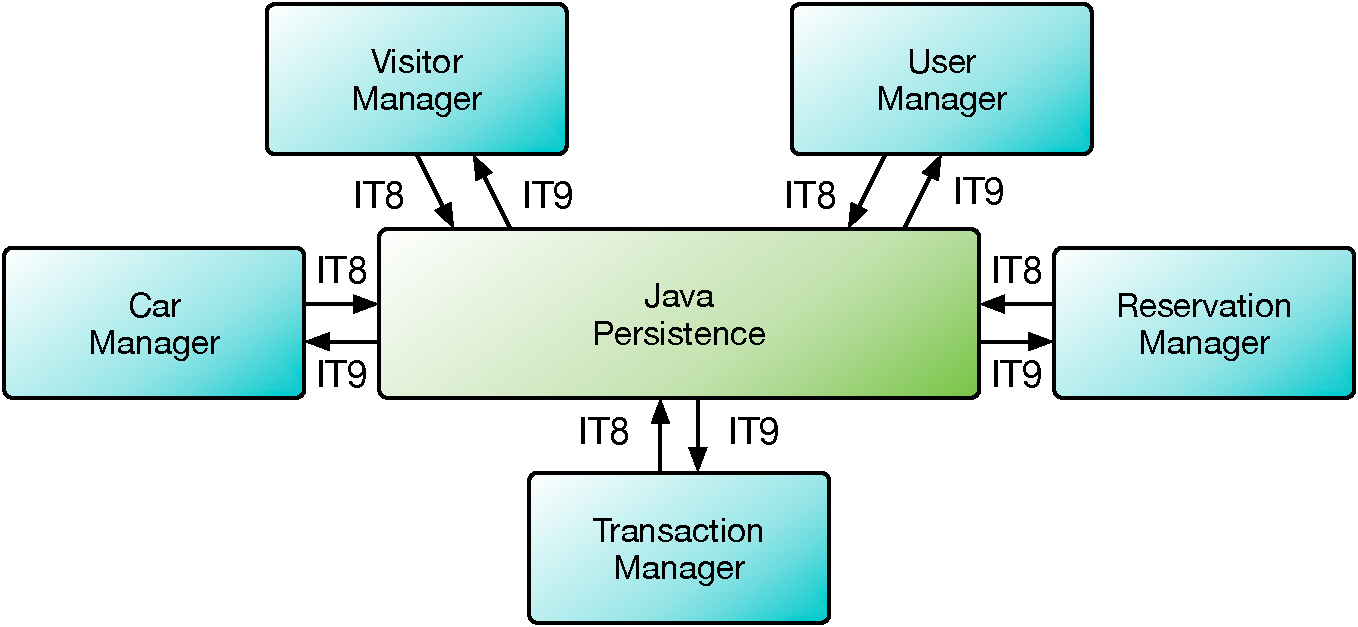
\includegraphics[width=0.9\textwidth]{Images/IT8-9-.pdf}
\vspace{16pt}
\caption{Business-tier subcomponents and Java Perstistence connections}
\label{fig:it8-9}
\end{figure}

\begin{table}[htbp]
\begin{center}
\begin{tabular}[t]{cccc}

\hline
\textbf{ID} & \textbf{Components} & \textbf{\acs{it}} & \textbf{\acs{tp}}\\
\hline
IT8 & \enspace User Manager $\rightarrow$ Java Persistence \enspace & \ref{sssec:IT8} & \ref{sssec:TP3}\\
\hline
IT8 & \enspace Visitor Manager $\rightarrow$ Java Persistence \enspace & \ref{sssec:IT8} & \ref{sssec:TP3}\\
\hline
IT8 & \enspace Car Manager $\rightarrow$ Java Persistence \enspace & \ref{sssec:IT8} & \ref{sssec:TP3}\\
\hline
IT8 & \enspace Reservation Manager $\rightarrow$ Java Persistence \enspace & \ref{sssec:IT8} & \ref{sssec:TP3}\\
\hline
IT8 & \enspace Transaction Manager $\rightarrow$ Java Persistence \enspace & \ref{sssec:IT8} & \ref{sssec:TP3}\\
\hline
IT9 & \enspace Java Persistence $\rightarrow$ User Manager \enspace & \ref{sssec:IT9} & \ref{sssec:TP3}\\
\hline
IT9 & \enspace Java Persistence $\rightarrow$ Visitor Manager \enspace & \ref{sssec:IT9} & \ref{sssec:TP3}\\
\hline
IT9 & \enspace Java Persistence $\rightarrow$ Car Manager \enspace & \ref{sssec:IT9} & \ref{sssec:TP3}\\
\hline
IT9 & \enspace Java Persistence $\rightarrow$ Reservation Manager \enspace & \ref{sssec:IT9} & \ref{sssec:TP3}\\
\hline
IT9 & \enspace Java Persistence $\rightarrow$ Transaction Manager \enspace & \ref{sssec:IT9} & \ref{sssec:TP3}\\
\hline

\end{tabular}
\caption{Business-tier subcomponents and Java Perstistence connections}
\end{center}
\end{table}

\clearpage

\vspace{120pt}
\begin{figure}[htbp]
\centering
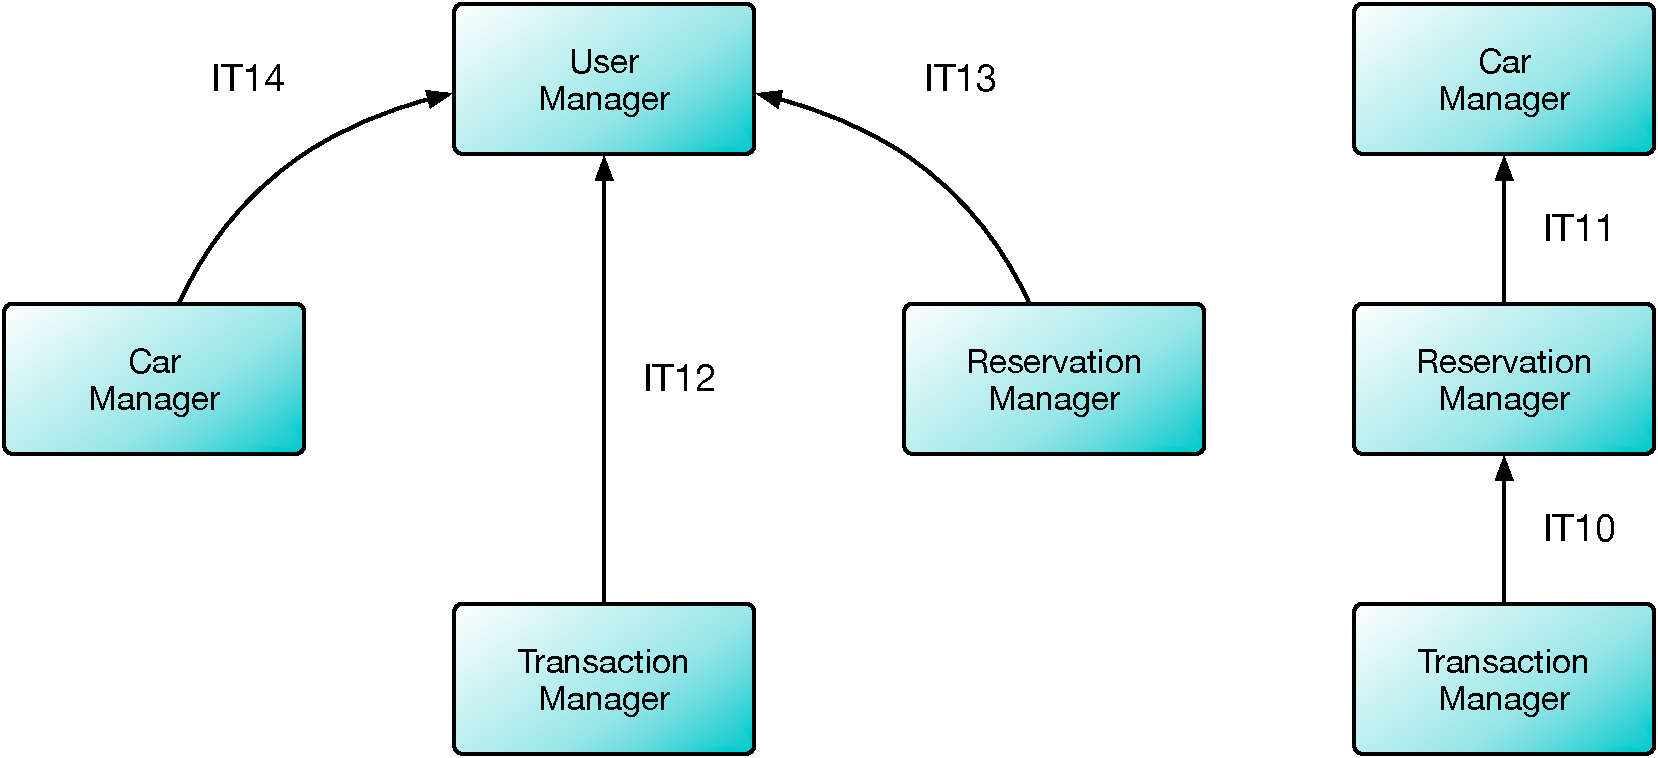
\includegraphics[width=\textwidth]{Images/IT10-14.pdf}
\vspace{16pt}

\label{fig:it10-14}
\caption{Business-tier subcomponents connections}
\end{figure}
\vspace{16pt}

\begin{table}[htbp]
\begin{center}
\begin{tabular}[t]{cccc}

\hline
\textbf{ID} & \textbf{Components} & \textbf{\acs{it}} & \textbf{\acs{tp}}\\
\hline
IT10 & \enspace Transaction Manager $\rightarrow$ Reservation Manager \enspace & \ref{sssec:IT10} & \ref{sssec:TP4}\\
\hline
IT11 & \enspace Reservation Manager $\rightarrow$ Car Manager \enspace & \ref{sssec:IT11} & \ref{sssec:TP4}\\
\hline
IT12 & \enspace Transaction Manager $\rightarrow$ User Manager \enspace & \ref{sssec:IT12} & \ref{sssec:TP4}\\
\hline
IT13 & \enspace Reservation Manager $\rightarrow$ User Manager \enspace & \ref{sssec:IT13} & \ref{sssec:TP4}\\
\hline
IT14 & \enspace Car Manager $\rightarrow$ User Manager \enspace & \ref{sssec:IT14} & \ref{sssec:TP4}\\
\hline

\end{tabular}
\caption{Business-tier subcomponents connections}
\end{center}
\end{table}

\clearpage

\vspace{120pt}

\begin{figure}[htbp]
\centering
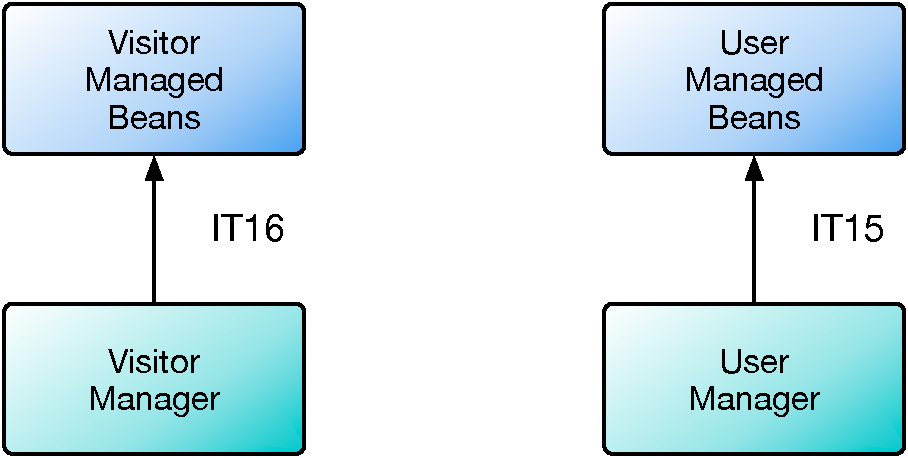
\includegraphics[width=0.6\textwidth]{Images/IT15-16.pdf}
\vspace{16pt}
\caption{Managed Beans and corresponding Managers connections}
\label{fig:it15-16}
\end{figure}

\vspace{16pt}

\begin{table}[htbp]
\begin{center}
\begin{tabular}[t]{cccc}

\hline
\textbf{ID} & \textbf{Components} & \textbf{\acs{it}} & \textbf{\acs{tp}}\\
\hline
IT15 & \enspace User  Manager$\rightarrow$ User Managed Beans \enspace & \ref{sssec:IT15} & \ref{sssec:TP5}\\
\hline
IT16 & \enspace Visitor Manager $\rightarrow$ Visitor Managed Beans \enspace & \ref{sssec:IT16} & \ref{sssec:TP5}\\
\hline

\end{tabular}
\caption{Managed Beans and corresponding Managers connections}
\end{center}
\end{table}

\clearpage